\documentclass[10pt]{article}
\newcommand{\HRule}{\rule{\linewidth}{0.5mm}}
\parindent 0pt
\parskip 10pt
\usepackage{anysize}
\usepackage{graphicx}
\usepackage{epsfig}
\usepackage{float}
%\usepackage{cite}
\usepackage{natbib}
\usepackage{setspace}
\marginsize{3.5cm}{3.5cm}{1cm}{1cm}
\onehalfspacing
\usepackage{caption}
\usepackage{subcaption}
\usepackage{amsmath,hyperref}

\usepackage{xcolor}
\hypersetup{
    colorlinks,
    linkcolor={red!50!black},
    citecolor={blue!50!black},
    urlcolor={blue!80!black}
}

%\textwidth 15cm
%\textheight 24cm
%\onehalfspacing
\begin{document}

\title{Bike Forecast}

\author{David Starkey}

\maketitle





\section{Introduction and Data Ingestion}
This project provides the details of bike hires in Montreal Canada dating from 2014 up to August 2017. The goal is to use statistical models to forecast the expected daily number of bike hires between two stations ( and ) for one weeks worth of hires between xxx and xxx. Each bike hire records the date, departure station and arrival station. This data is contained within several csv files which collectively total 15.3 million entries.

This summary is presented as follows. Section xx details the data ingestion process. Section xx presents the findings of the initial exploratory data analysis and includes several figures that motivate the model fitted to the global sample discussed in Section xxx. The results of the model fitting are provided in Section xxx.


\section{Data Ingestion}
\label{sec_ingest}



\section{Exploratory Data Analysis}
\label{sec_exp}

\subsection{Time Series}
Before deciding how best to model the forecasting problem, a universally sound first step is to visualise the data. I use Pythons matplotlib module to plot the number of bike hires as a time series, concatenating all four years of observations together. Figure \ref{fig_ts} presents some very important information on the Time Series

\begin{itemize}
\item The time series is periodic. It exhibits a similar annual pattern with bike hires becoming more popular in the summer months.

\item The amplitude of the variations appears to be increasing over time (smooth red line Figure \ref{fig_ts}). This suggests bike hires are increasing in popularity.
\end{itemize}




\begin{figure}
\begin{center}
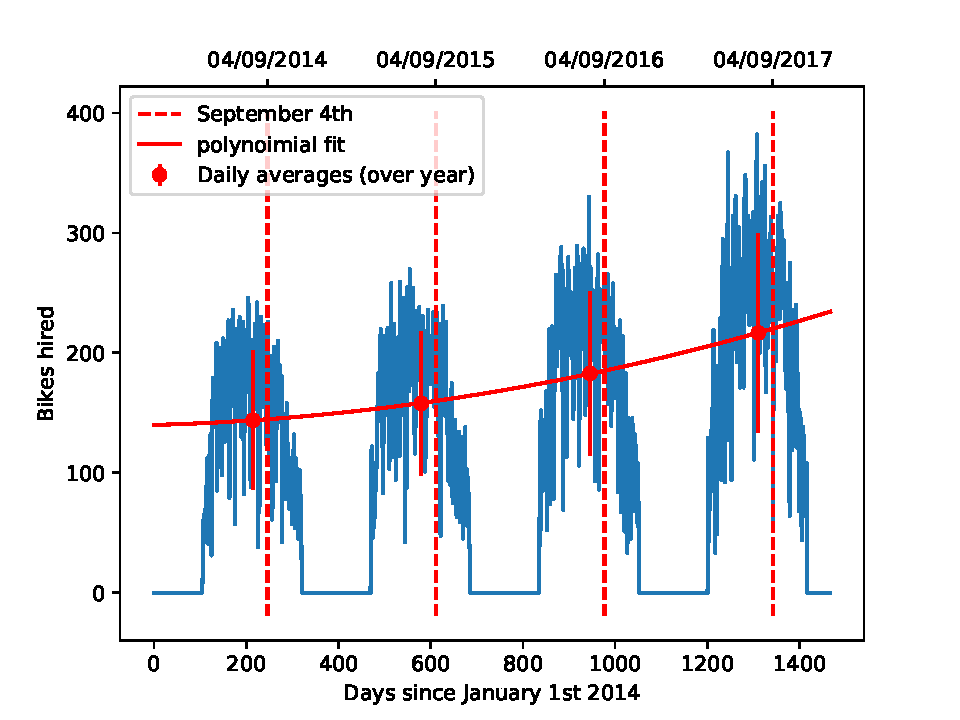
\includegraphics[scale=1.0,angle=0,trim=0cm 0cm 0cm 0cm]{ts_plot.pdf}
\caption{Time series of bike hires. Y axis plots the number of bikes hired per day as a function of day number (days are measured relative to 1st January 2014). The vertical red dashed lines show 4th September of each year (the start of the forecast week) and the smooth vertical polynomial fit shows how the average daily number of bike hires increases over the four years of data.}
\label{fig_ts}
\end{center}
\end{figure}
\begin{figure}
\begin{center}
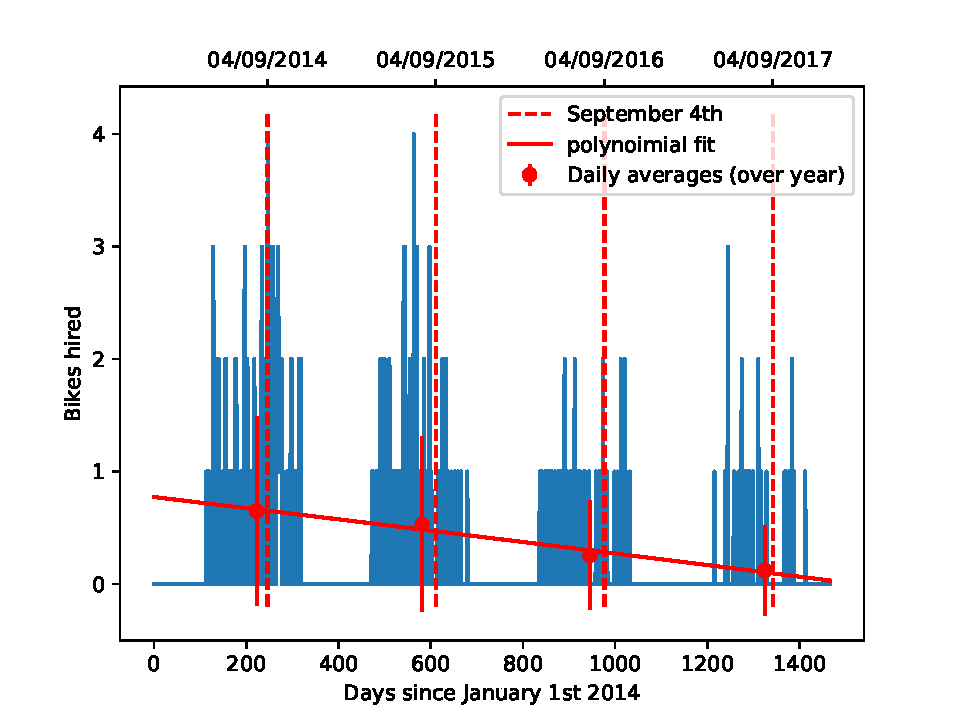
\includegraphics[scale=1.0,angle=0,trim=0cm 0cm 0cm 0cm]{ts_plot_station.pdf}
\caption{Same as Figure \ref{fig_ts} but restricting the time series only to bike hires departing at station xx and ending at station xx}
\label{fig_ts_station}
\end{center}
\end{figure}




While Figure \ref{fig_ts} provides useful information on the periodicity of the time series, this information is much clearer to see when presented as a power spectrum. The power spectrum as a function of frequency $P(f)$ can be computed from the fourier transform of time-series data $F(f)$ where

\begin{equation}
\label{eq_ft}
F(f) = \int_{-\infty}^{\infty} f(t) e^{-2\pi f t} dt,
\end{equation}
\noindent and $P(f)$ is then

\begin{equation}
\label{eq_ps}
P(f) = F^*(f) F(f),
\end{equation}

\noindent where $*$ denotes complex conjugation. Qualitatively, the power spectrum $P(f)$ tells us if there are strong periodic features in our data set. Figure \ref{fig_ps} demonstrates that the bike hires in this data set go through seasonal and weekly cycles of popularity, likely due to the seasonal weather / holiday season and weekend trend increases.





\begin{figure}
\begin{center}
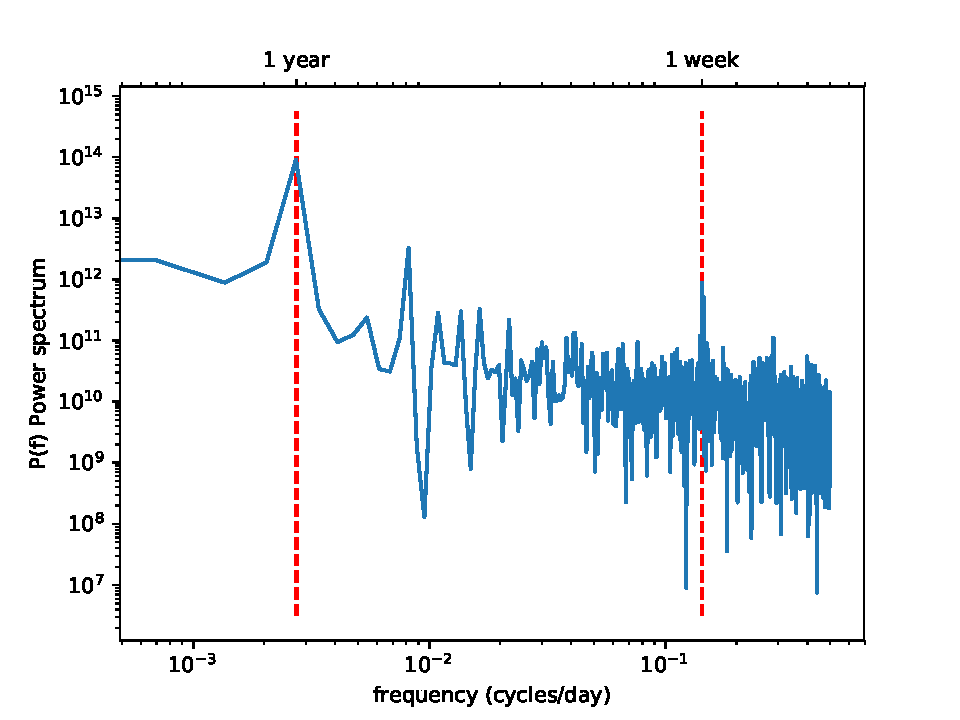
\includegraphics[scale=1.0,angle=0,trim=0cm 0cm 0cm 0cm]{ps_plot.pdf}
\caption{Power spectrum $P(f)$ versus frequency of the time series data presented in Figure \ref{fig_ts}. The peaks at one year and one week timescales (red dashed lines) show that bike hire goes through seasonal and weekly cycles of popularity.}
\label{fig_ps}
\end{center}
\end{figure}






\section{Model fitting (Recurrent Neural Network)}
\label{sec_recur}


Now that the periodicity of the bike hires is better understood, I will fit a model to the global sample to forecast the bike hires for the week beginning 4th September 2017. The model I use here is known as a recurrent neural network (RNN). Unlike the multi-layer-perceptron, RNN's are specialised types of neural networks that excel at modeling time-series data. This makes them excellent forecasting tools. Before describing the mathematics and architechture of RNN's, I first give a bried introduction to the simplest kind of neural net (the multi-layer-perceptron). Many of the features and concepts are interchangeable between the two and it is hoped that, once the MLP is described here, it will help to understand the statistics and principles behind the RNN.



\subsection{Mulit-Layer-Perceptron (MLP)}

\subsection{Theory} 


In its simplest form, a neural network is composed of a single ($j=1$) `neuron'. This neuron takes an arbitrary number of $i$ input values, each modulated by a `weight' parameter $W_{ij}$ \footnote{Much of the theory in this section can be found in most texts on neural networks but wikipedia does a good job explaining the mathematical detail \href{ https://en.wikipedia.org/wiki/Backpropagation}{\textcolor{blue}{https://en.wikipedia.org/wiki/Backpropagation}}, as do the online Stanford lecture series' \href{ https://www.coursera.org/lecture/machine-learning/backpropagation-algorithm-1z9WW}{\textcolor{blue}{https://www.coursera.org/lecture/machine-learning/backpropagation-algorithm-1z9WW}}}. The weighted sum of these is known as the `activation' $z$ and is operated on by the neuron with an activation function $f (z)$ to yield an output quantity $a$. The output from the entire neural network for an input data example vector $\vec{X}_n$ (in situations with a chain of neurons as is the case later) is denoted $h(W,\vec{X}_n)$. A back propagation approach is used to optimize the weights (detailed below) in multi layer neural networks. This requires that the activation function $f(z)$ be differentiable. In this project (as is common for many neural networks), a sigmoid activation function is adopted where 

\begin{equation} 
f(z) = \frac{1}{1+e^{-z}},
\label{eq_sigmoid}
\end{equation}

\noindent with a derivative

\begin{equation} 
f`(z) = f(z) \left( 1 - f(z) \right).
\label{eq_sigmoid}
\end{equation}


\noindent This activation function always returns a number between 0 and 1. Once the weights are optimised, the neuron will output a value close to 0 to indicate one class, and close to 1 to indicate the other. The mathematical rigour in neural networks is in the weight-optimisation step. 


\begin{figure}
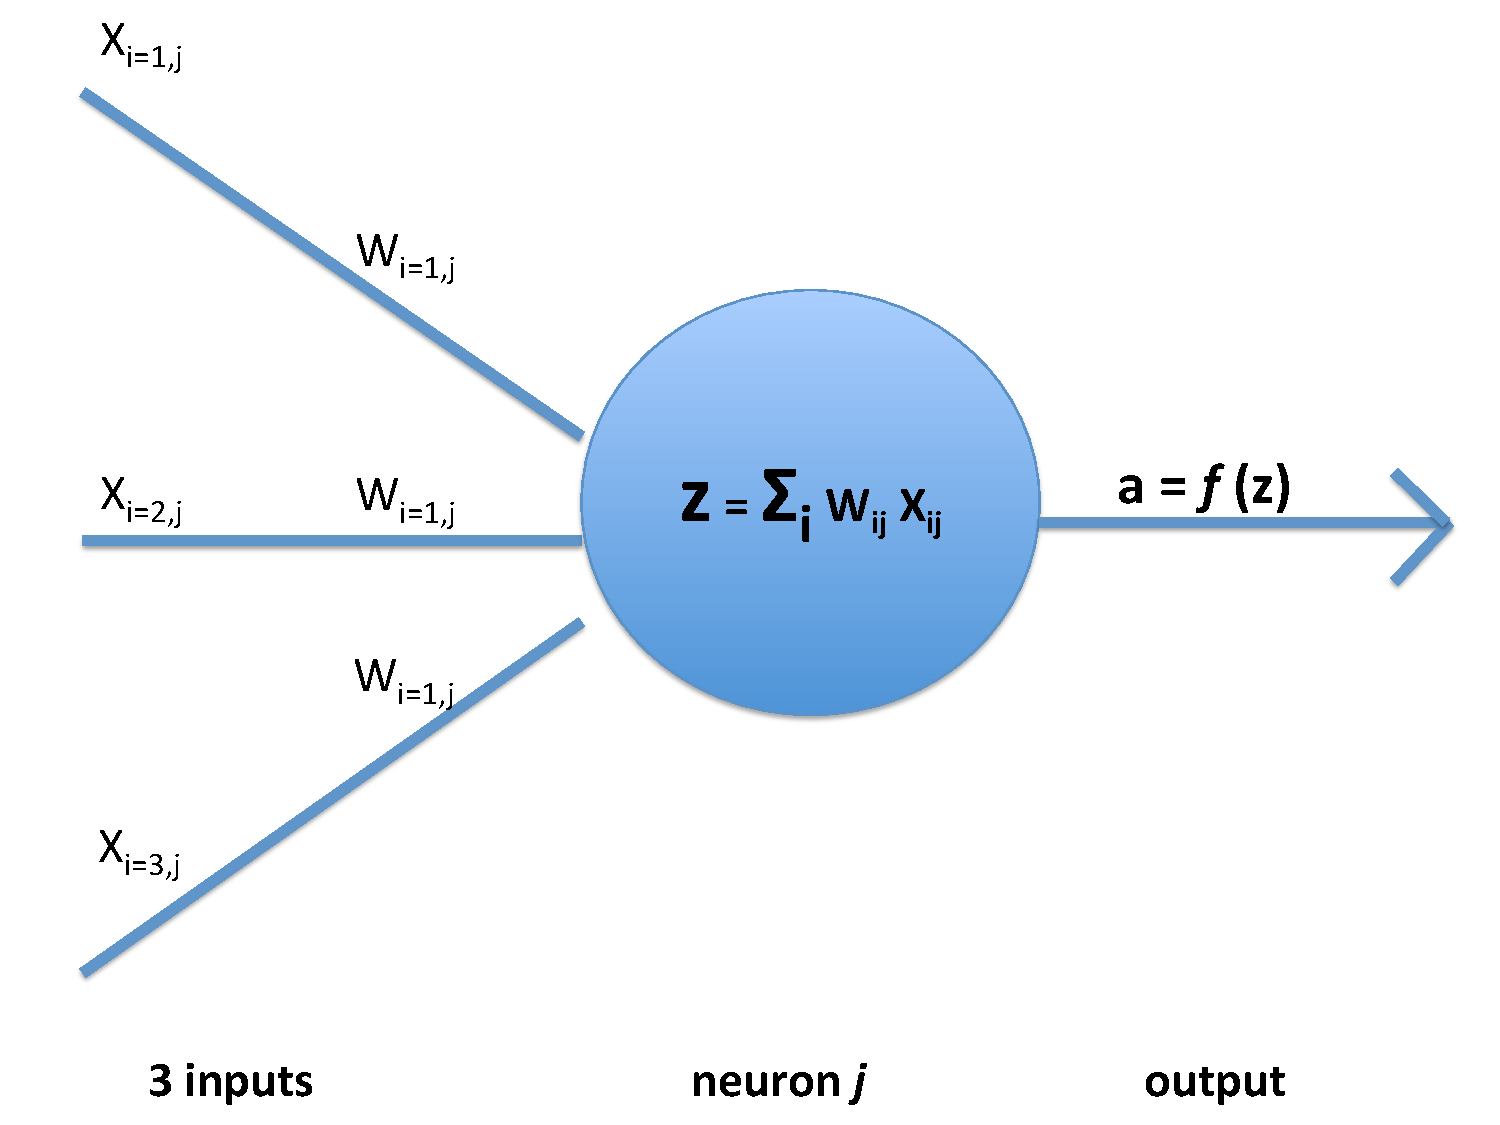
\includegraphics[scale=0.5,angle=0,trim=0cm 0cm 0.0cm 0cm]{diagrams.pdf}
\caption{Example neural network with a single neuron. The network has three inputs to neuron $j$ denoted by $X_{ij}$ with weights $W_{ij}$. The output from the neuron is given by $a_j$ where the activation function $f(z)$ is given in Equation \ref{eq_sigmoid}.}
\label{fig_temp}
\end{figure}


\subsection{optimizing the weights}

Like many optimisation problems, I start with the cost function (often called $\chi^2$ or the error function). For a single (or multi) layer neural network, this takes the form.

\begin{equation}
J(W) = \frac{1}{N} \sum_{n=1}^N \frac{ \left( h(W,\vec{X}_n) - y_n \right)^2} {2}
\label{eq_cost}
\end{equation}

\noindent where $y_n$ denotes the classification of the $n$th training sample of $N$ total samples with an input data vector $\vec{X}_n$.



The back propagation algorithm works using the principle of gradient descent. This iteratively updates each weight until the cost function is minimised. After one iteration, the weight $W_{ij}$ is adjusted according to 

\begin{equation}
W_{ij} = W_{ij} - \alpha \frac{\partial}{\partial W_{ij}} J\left( W \right),
\label{eq_adjust_w}
\end{equation}



\noindent where $\alpha$ is the learning rate. A high value $>1$ for the learning rate will encourage the weight parameter to take large steps as it is optimized. This has the potential advantage of reducing the convergence time but may cause the global minimum to be missed and lead inaccurate weights.

The partial derivative of the total cost function $\frac{\partial}{\partial W_{ij}} J\left( W \right)$ depends on the partial derivatives of each of the $N$ training examples like 

\begin{equation}
\frac{\partial}{\partial W_{ij}^{(l)}} J(W,b) = \left[ \frac{1}{N} \sum_{i=1}^N \frac{\partial}{\partial W_{ij}^{(l)}} J(W; \vec{x_i}, y_i) \right], 
\label{eq_partial_tot}
\end{equation}


\noindent and the partial derivatives for the individual weight parameters $\frac{\partial}{\partial W_{ij}^{(l)}} J(W; \vec{x_i}, y_i)$ are given by 



\begin{equation}
\frac{\partial}{\partial W_{ij}} J\left( W \right) = a_j^l \delta_i^{l+1},
\label{eq_partdiv}
\end{equation}

\noindent where $a_j^l$ corresponds to the output from neuron $j$ in level $l$. The intermediate error function $\delta_i^{l+1}$ calculates how responsible the $i$th neuron in layer $l$ is for errors in the output. $\delta$ depends on the level of the neuron in the network. For an outer level neuron in layer $l=n_l$,

\begin{align}
\delta^{(n_l)}_i
= \frac{\partial}{\partial z^{(n_l)}_i} \;\;
\frac{1}{2} \left\|y - h_{W,b}(x)\right\|^2 = - (y_i - a^{(n_l)}_i) \cdot f'(z^{(n_l)}_i),
\label{eq_delta}
\end{align}


\noindent and for an inner level neuron

\begin{equation}
\delta^{(l)}_i = \left( \sum_{j=1}^{s_{l+1}} W^{(l)}_{ji} \delta^{(l+1)}_j \right) f'(z^{(l)}_i).
\label{eq_delta_in}
\end{equation}


Combining Equations \ref{eq_partial_tot} through \ref{eq_delta_in} with Equation \ref{eq_adjust_w} and iterating will encourage the weights toward their optimal values and minimize the cost function (Equation \ref{eq_cost}).




\subsection{Recurrent Neural Network}
Now that the MLP has been introduced, understanding the RNN is much more intuitive. The goal is to optimize the weights and minimize the cost function as with the MLP. The only difference now is to note that RNN's are specialised for dealing with time series data where subsequent data points depend on previous points. The periodic nature of the time series data in Figure \ref{fig_ts} shows that this is such a situation. The cyclic pattern of rising and falling popularity with bike hires allows us to forecast the demand in future. To captialize on the deterministic time series features, we need a neural network with a slightly different design. Figure \ref{fig_rnn} shows the layout of an RNN. Minimizing the cot function Equation \ref{eq_cost} proceeds in the same way as the MLP and the back propagation works by starting from the latest point in the time series and working in (from right to left in Figure \ref{fig_rnn}).



\begin{figure}
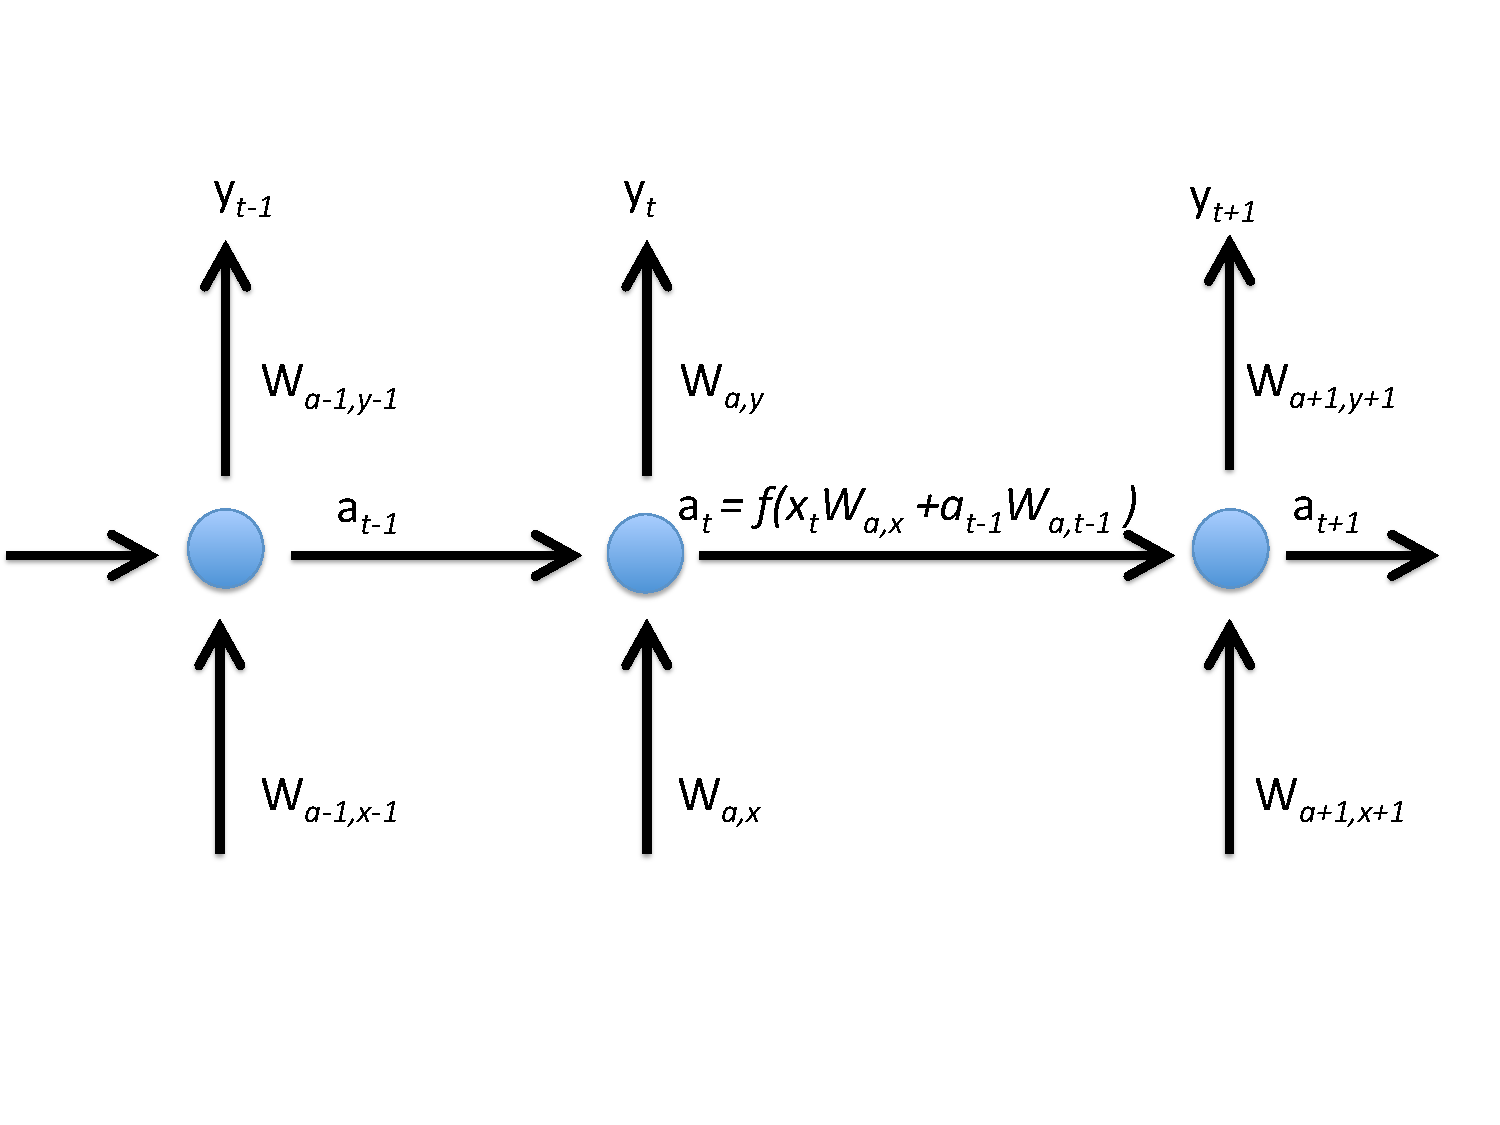
\includegraphics[scale=0.5,angle=0,trim=0cm 0cm 0.0cm 0cm]{rnn.pdf}
\caption{Diagram showing architecture of an RNN. Rather than side by side as with a MLP, each neuron appears sequentially. Additionally an RNN produces an output $y$ at each neuron rather than just a single output at the end of the network. The activation function $f$ takes the same form as Equation \ref{eq_sigmoid} used in the MLP, and the weights $W$ are updated using a back propagation algorithm similar to Equation \ref{eq_adjust_w}.}
\label{fig_rnn}
\end{figure}


\section{Results}
\label{sec_results}
The RNN is trained on the time series observations (Figure \ref{fig_ts}) up to the 3rd September 2017. The remaining entries in the csv file serve only as a bench mark test data set to test the RNN's accuracy. In Figure xx, I first use the entire of the 2017 entries as the test data set to illustrate the predictive power of the RNN (in other words the model sees no data from 2017). Figure xx shows that the RNN is able to forecast the entire frequency of bike hires for the whole of 2017 and is able to replicate many of the observed features quite remarkably.




Given the objective here is to predict the freqwuency of bike hires only between stations xx and xx, one could train the RNN using only entries between these stations. However, Figure xx shows that this would throw out almost all of the data and leave only a very small number of samples on which to train the network. 







\end{document}